Since the pendulum relation uses SI units, each length is first converted from millimetres to metres. For set \(j\), the relation from A.1 then gives

\[\boxed{\omega_{n,j}=\sqrt{\frac{g}{L_j}}}\qquad\text{(A.2.1.a)}\]

The frequency and period follow from \(\omega_{n,j}=2\pi f_{n,j}\) and \(f_{n,j}=1/\tau_j\), so

\[\boxed{f_{n,j}=\frac{\omega_{n,j}}{2\pi}}\qquad\text{(A.2.1.b)}\]

\[\boxed{\tau_j=\frac{2\pi}{\omega_{n,j}}}\qquad\text{(A.2.1.c)}\]

Using \(g=9.81\ \mathrm{m/s^2}\) and the ten lengths gives the following values for A.2.1.d.

{ % do not increment counter
\begin{center}\small\begin{tabular}{@{}rrrrr@{}}
\toprule\noalign{}
Set & \(L\) (mm) & \(\omega_n\) (rad/s) & \(f_n\) (Hz) & \(\tau\) (s) \\
\midrule\noalign{}
1 & 561.535 & 4.18 & 0.665 & 1.503 \\
2 & 562.691 & 4.18 & 0.665 & 1.505 \\
3 & 563.845 & 4.17 & 0.664 & 1.506 \\
4 & 563.845 & 4.17 & 0.664 & 1.506 \\
5 & 565.000 & 4.17 & 0.663 & 1.508 \\
6 & 565.000 & 4.17 & 0.663 & 1.508 \\
7 & 566.155 & 4.16 & 0.663 & 1.509 \\
8 & 566.155 & 4.16 & 0.663 & 1.509 \\
9 & 567.309 & 4.16 & 0.662 & 1.511 \\
10 & 568.464 & 4.15 & 0.661 & 1.513 \\
\bottomrule\end{tabular}\end{center}
}

The mean of each calculated column follows from \(\overline{q}=\frac{1}{10}\sum_{j=1}^{10}q_j\). Therefore, the values required in A.2.2 are

\[\boxed{\overline{\omega_n}=4.17\ \mathrm{rad/s}}\qquad\text{(A.2.2)}\]

\[\boxed{\overline{f_n}=0.663\ \mathrm{Hz}}\qquad\text{(A.2.2)}\]

\[\boxed{\overline{\tau}=1.508\ \mathrm{s}}\qquad\text{(A.2.2)}\]

For A.2.3, the initial velocity is zero, so the A.1 response reduces to

\[\boxed{u(t)=u_0\cos(\overline{\omega_n}t)=2\cos(4.166893t)\ \mathrm{mm}}\qquad\text{(A.2.3)}\]

At \(t_1=10\ \mathrm{s}\), substitution into the response gives

\[\boxed{u(t_1)=2\cos\!\left(4.166893\times10\right)\ \mathrm{mm}=-1.352\ \mathrm{mm}}\qquad\text{(A.2.3.a)}\]

For the requested ten-cycle duration, multiply the mean period by \(N_{\mathrm{osc}}=10\). The duration and corresponding position are

\[\boxed{t_{N_{\mathrm{osc}}}=10\overline{\tau}=15.08\ \mathrm{s}}\qquad\text{(A.2.3.b)}\]

\[\boxed{u_{N_{\mathrm{osc}}}=u(10\overline{\tau})=2.000\ \mathrm{mm}}\qquad\text{(A.2.3.b)}\]

The mean of the individual periods is \(\overline{\tau}=1.5078872528\ \mathrm{s}\), whereas the period associated with the mean frequency is \(2\pi/\overline{\omega_n}=1.5078825285\ \mathrm{s}\). Averaging and taking a reciprocal do not commute. Following the prompt, the duration uses \(10\overline{\tau}\); the difference from ten exact cycles of the mean-frequency model is only \(47.2\ \mu\mathrm{s}\), and the endpoint still rounds to \(2.000\ \mathrm{mm}\).

Using the boxed A.2.3 expression over \(0\leq t\leq10\overline{\tau}\) gives the ten-oscillation response below. Since the marker is placed at \(t_1=10\ \mathrm{s}\), the plotted value is

\[\boxed{u(10)=-1.352\ \mathrm{mm}}\qquad\text{(A.2.3.c)}\]

\begin{figure}[H]
\centering
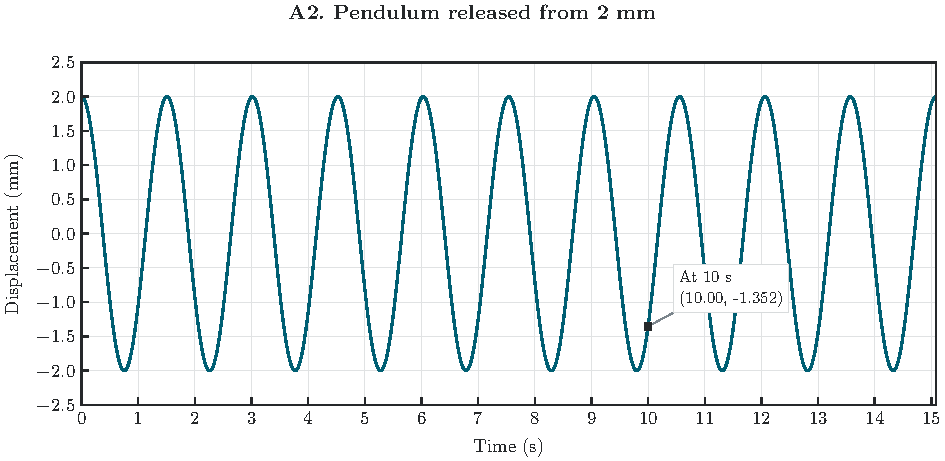
\includegraphics[width=0.95\linewidth,height=\textheight,keepaspectratio,alt={A.2.3.c. Pendulum response over ten oscillations with a data tip at ten seconds.}]{figures/generated/solutions/A2.pdf}
\caption{A.2.3.c. Pendulum response over ten oscillations with a data tip at \ensuremath{t=10\,\mathrm{s}}.}
\end{figure}

\clearpage
\matlabcaption{Script used to reproduce Figure~4.}

\lstinputlisting[style=hwmatlab]{matlab/A2.m}
